%!TEX root = ../thesis.tex

\thispagestyle{myheadings}

\graphicspath{{Body/Figures/TrackingFigures/}{Body/Figures/TrackingFigures/MainPlots/}{Body/Figures/TrackingFigures/MainPlots/PlanePlots/}{Body/Figures/TrackingFigures/MainPlots/PullPlots/}{Body/Figures/TrackingFigures/MainPlots/Residuals/}{Body/Figures/TrackingFigures/eLoss/}{Body/Figures/TrackingFigures/CoordSys/}{Body/Figures/TrackingFigures/TrackerPics/}{Body/Figures/TrackingFigures/Field/}{Body/Figures/TrackingFigures/TrackingFlow/}{Body/Figures/TrackingFigures/LeftRight/}{Body/Figures/TrackingFigures/Misc/}{Body/Figures/TrackingFigures/Extrapolation/}{Body/Figures/TrackingFigures/Tracks/}{Body/Figures/TrackingFigures/BeamMeasurements/}{Body/Figures/TrackingFigures/MCDataComparison/}}

\chapter{Track Reconstruction and Analysis}
\label{chapter:TrackReconstruction}

As described in section \ref{sec:StrawTrackers}, the straw trackers are used to provide information about the muon beam, important for the calorimeter \wa analysis, calculating the \wa pitch correction, and determining the spatially weighted magnetic field seen by the muons. The track reconstruction is performed in three stages: First, individual hits in the tracker are grouped into individual tracks in the finding stage. Second, a best trajectory is fit to grouped hits in the fitting stage. Third, the best fit trajectory is extrapolated back to the storage region or forwards to the calorimeter in the extrapolation stage. A fourth refinement stage is planned but not yet implemented, which would add or remove hits in the finding stage based on the results of the fitting and extrapolation stages.

As a brief aside, every stage of the track reconstruction is performed in the event-processing framework known as \textit{art} \cite{art}. The \textit{art} framework is a collection of modularized stages in a C++ framework useful for reading, reconstructing, filtering, analyzing, and writing data, among other things. All Fermilab experiments now use \textit{art}, and E989 is no exception.


\section{Track Finding}
\label{sec:TrackFinding}

The track finding stage consists of pattern recognition routines in order to group individual hits into separate sets corresponding to individual incident tracks. The general implementation of these pattern recognition routines is relatively straightforward \cite{trackfinding,trackfinding2}. Hits across all modules are grouped in time windows called time islands, with a max width of $\SI{100}{ns}$. Within those time islands hits are then grouped into clusters. Clusters consist of one or two hits for each U or V view per module. As a reminder the U and V views of a module consist of the two U or V layers in that module, \secref{sec:StrawTrackers}. Hits are only clustered if they lie in close proximity in time and space to one another. The spatial constraint is defined as the difference in hit straw numbers, from 0 to 31 for the 32 straws per layer, which by default is limited to less than or equal to 4. Neighboring hit clusters in the same module are then grouped to form seeds, one per module. Finally, seeds in successive modules are grouped starting from one end of the tracker to form what are called track candidates. The seeds are formed and grouped into track candidates again only if they lie close in time and space to one another. The entire track candidate formation process occurs for all hits in a time island to find as many real tracks as possible. See \figref{fig:TrackCandidateSelection}.

After a track candidate has been formed a number of checks are made before passing it on to the fitting stage. If hits, clusters, or seeds are found to be shared among multiple track candidates, the candidates are dropped. Likewise, a track candidate is dropped if it is made from seeds consisting of only one type of view, or if the track candidate has less than six hits. There are also various small geometry and timing algorithms to improve the track candidates, such as removing hits from secondaries \cite{trackfinding3}. The $t_{0}$ time for the track candidate is calculated as the mean time of all hits, with some fixed offset at the end. This $t_{0}$ is helpfully constrained by geometry effects, where for a straight track passing through two layers in the same view, the sum of the drift times adds up to a constant (cite or show this?). The track candidate is supplied with an original momentum and position guess at the start of the track by fitting a circle to the hit straw wires in the horizontal plane. The final track candidates are passed on to the fitting stage. 


\begin{figure}[]
    \centering
    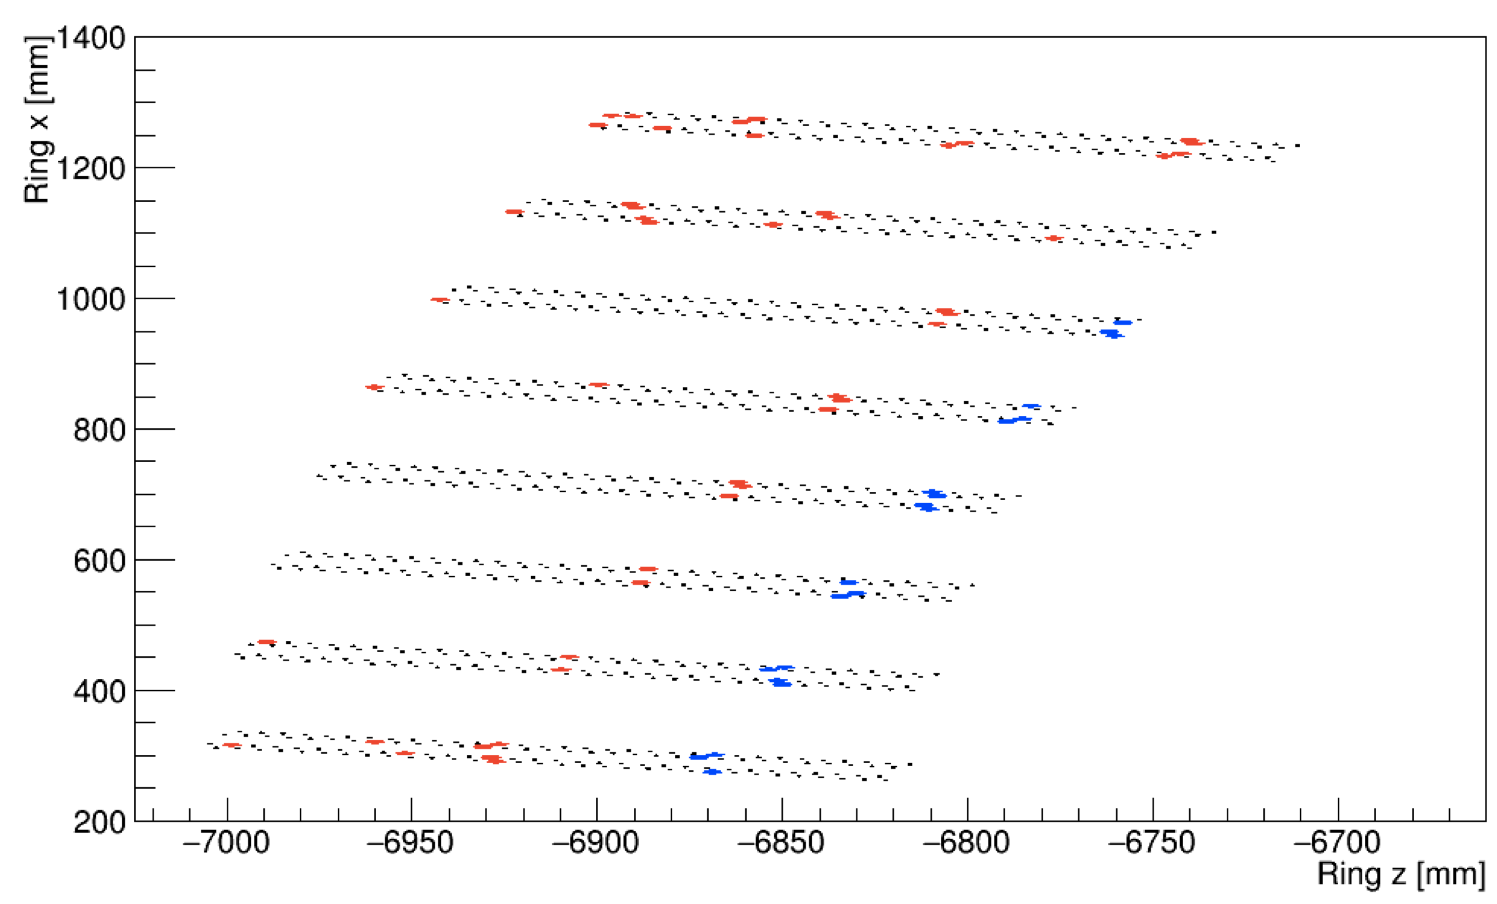
\includegraphics[width=0.9\textwidth]{TrackCandidateSelection}
    \caption[Track candidate selection]{Hits in a tracker station in a single time island. The black dots indicate the position of the straws, while the blue and red points indicate hits. In blue is the first formed track candidate in the island, formed from separate seeds in different modules. The track finding algorithms will move onto the remaining hits in the time island to attempt to form other track candidates, one of which is easily observable by eye.}    
    \label{fig:TrackCandidateSelection}
\end{figure}

% event display tracks

% \begin{figure}[]
% 	\centering
% 	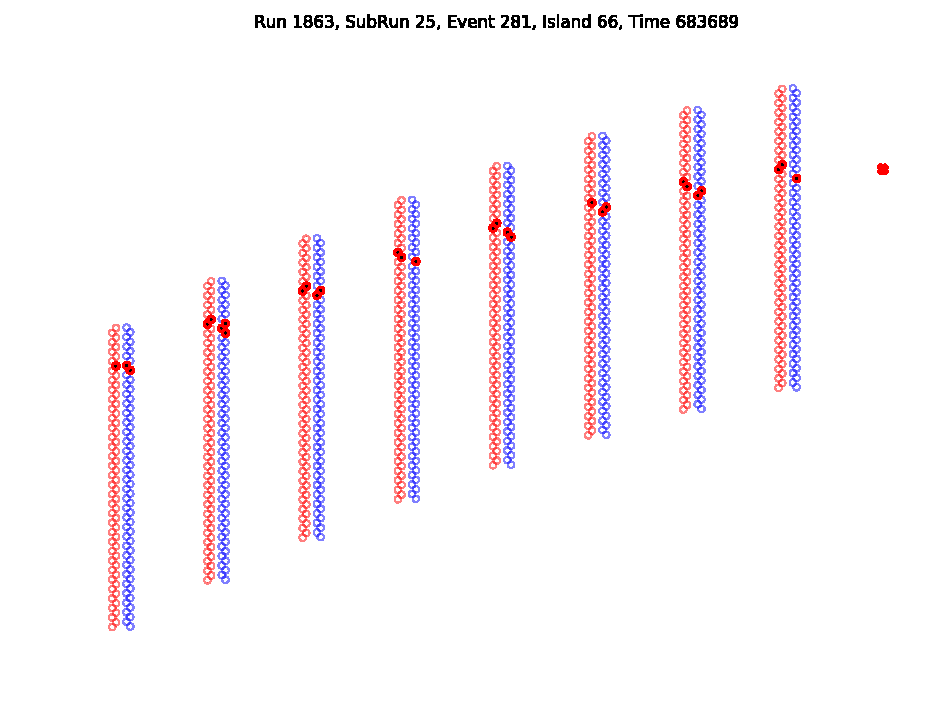
\includegraphics[width=0.9\textwidth]{TrackAndCaloHit}
%     \caption[TrackAndCaloHit]{clean up and possibly replace}    
%     \label{fig:TrackAndCaloHit}
% \end{figure}

% \begin{figure}[]
% 	\centering
% 	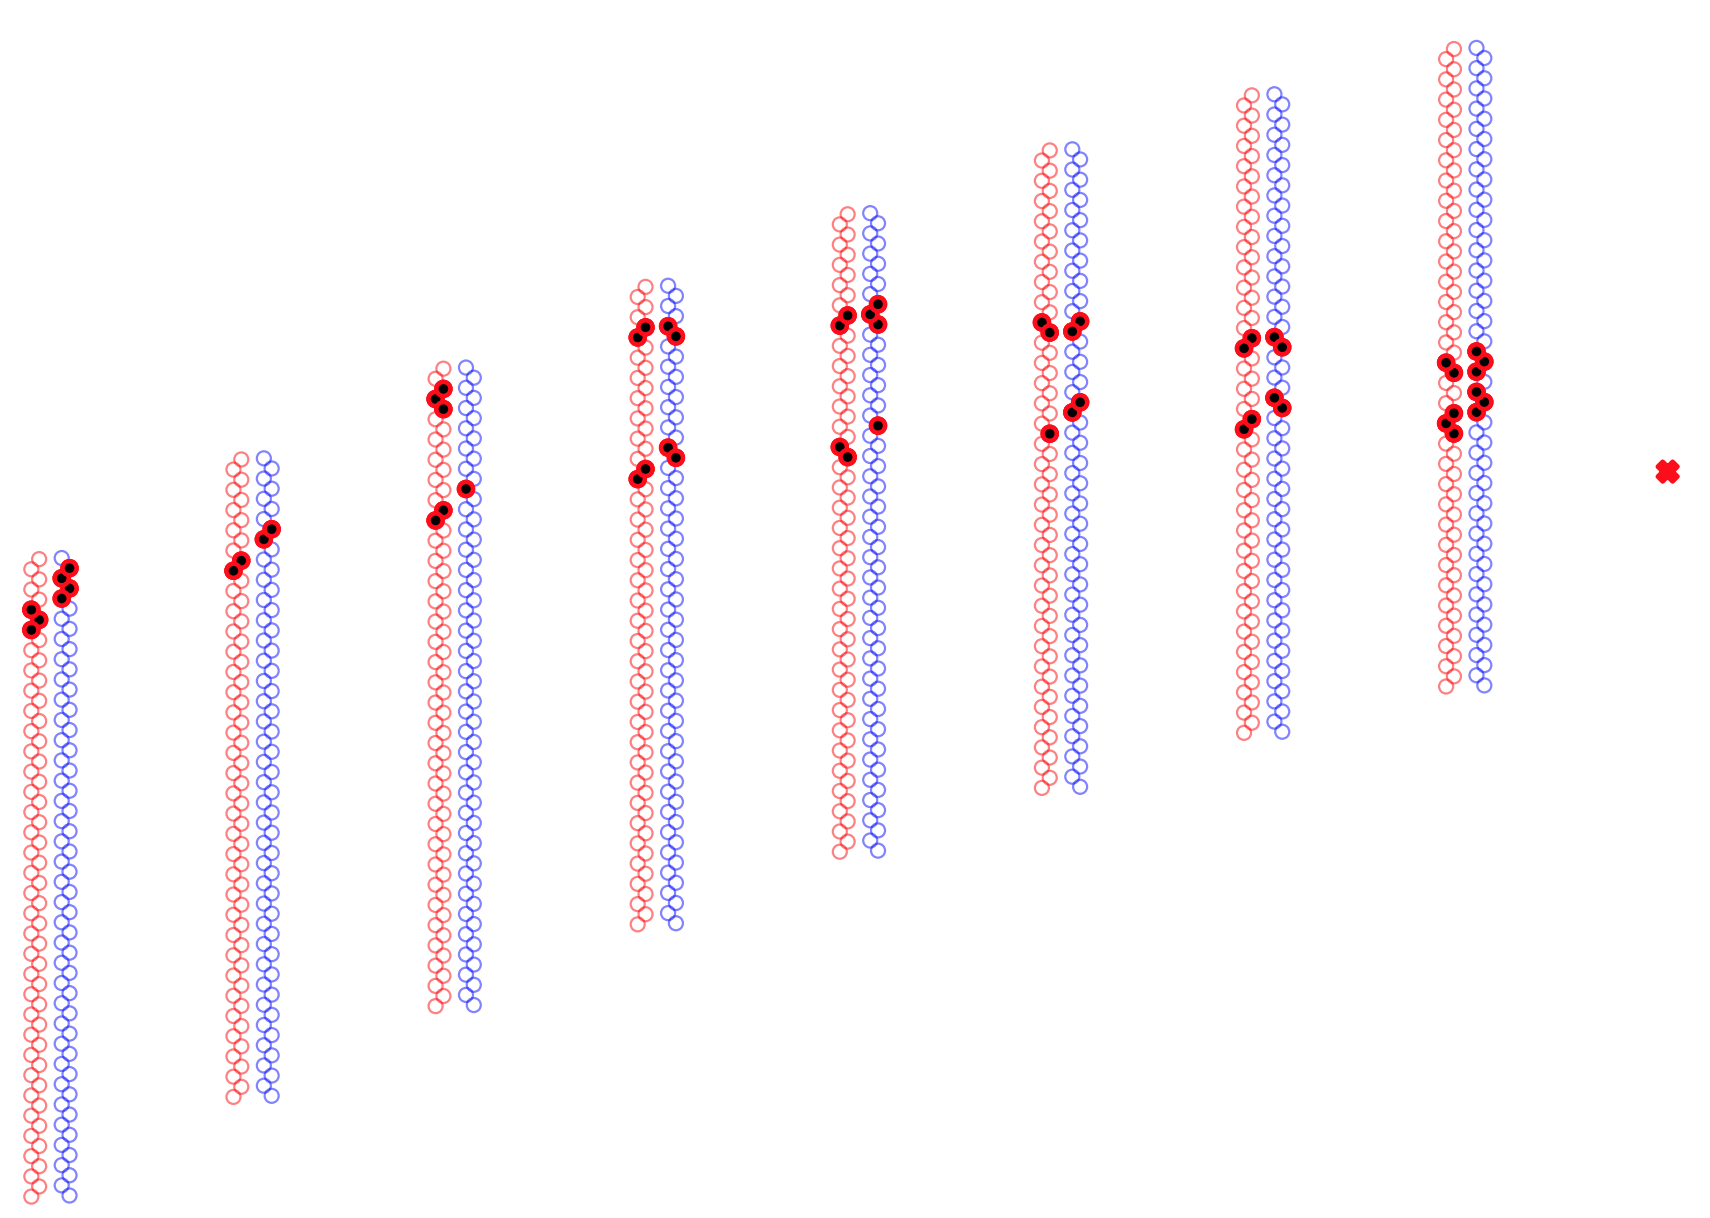
\includegraphics[width=0.9\textwidth]{pileupEvent}
%     \caption[pileupEvent]{clean up and possibly replace}    
%     \label{fig:pileupEvent}
% \end{figure}



\section{Track Fitting}
\label{sec:TrackFitting}


The track fitting stage takes the track candidates from the track finding stage, and outputs a best fit trajectory to those candidates. This includes optimal state vectors and error matrices for the track at each measurement plane and at a ficticious starting plane at the entrance to the straw tracking detector. The track fitting routines can roughly be split into two parts, error propagation and the actual fitting and improvement of the track. The implementation of these parts go hand in hand, and will be described in turn. 


\subsection{Error propagation and coordinate systems}
\label{sub:Geane}

To put it simply, the process of error propagation involves taking track parameters and error matrices (which describe the spread in those track parameters) and transporting them along discrete steps from one point to another, accounting for changes due to any present magnetic fields or material along the step path. There is a set of error propagation routines originally written in Fortran by the EMC collaboration, called ``Geometry and Error Propagation'' or Geane \cite{geanemanual}. Geane works by propagating particles along their average trajectories neglecting the effects of discrete processes, using a helix equation along small enough steps where the change in the magnetic field is small. These routines were used in the E821 experiment as well as the PANDA and FINUDA experiments with some success \cite{Lavezzi}. The Geane routines were at one point converted to C++ and added to Geant4. The strength of using Geane within a Geant4 simulation lies in its direct access to the Geant4 geometry and field. This is crucially important for the E989 track fitting because the trackers live in a region of high field non-uniformity. Shown in \figref{fig:Opera2DFields} is the location of the tracker with respect to the radial and vertical fields. As shown the radial field in the tracker region rises from $\SI{0}{T}$ at the outer ends to roughly $\SI{.3}{T}$ at the inner top and bottom ends, and the vertical field drops approximately 50\% from the storage dipole field of $\SI{1.451}{T}$. These large field gradients over the tracking measurement space must be handled appropriately, which Geane does nicely.



\begin{figure}[]
\centering
    \begin{subfigure}[]{0.75\textwidth}
        \centering
        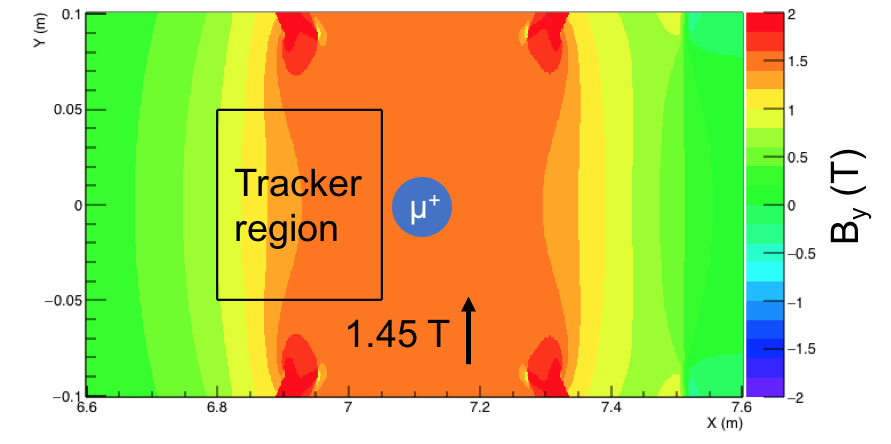
\includegraphics[width=\textwidth]{operaByMod}
        \caption{Vertical magnetic field}
    \label{fig:operaBy}
    \end{subfigure}%
    \vspace{5mm}
    \begin{subfigure}[]{0.75\textwidth}
        \centering
        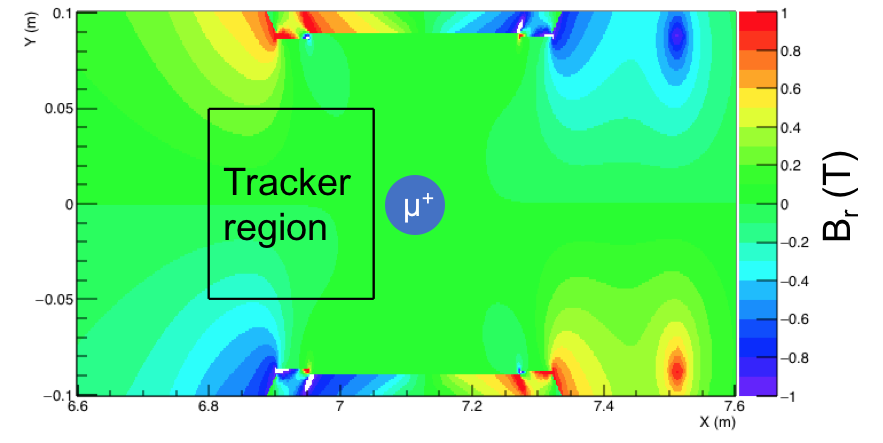
\includegraphics[width=\textwidth]{operaBxMod}
        \caption{Radial magnetic field}
    \label{fig:operaBx}
    \end{subfigure}
\caption[Vertical and radial magnetic fields calculated in Opera2D]{Shown are the vertical (top) and radial (bottom) magnetic fields of the storage ring magnet in and around the storage region as calculated in Opera 2D. The horizontal and vertical axes are the radial and vertical coordinates of the ring respectively. The center of the storage region lies at $\SI{7.112}{m}$ along the horizontal axis. The contours represent the strengths of the vertical and radial magnetic fields. The black box shows the rough location of the tracker with respect to the ring. It can be seen that there is a large field non-uniformity within the tracker space.}
\label{fig:Opera2DFields}
\end{figure}


Predicted track parameters in Geane are a function of path length 
        \begin{align} \label{eq:pp}
            p_{l} = F_{l,l_{0}}(p_{0}),
        \end{align}
where $p_{0}$ are some original tracker parameters and $p_{l}$ are the updated ones. The path length $l$ can be defined or limited how one wishes, and typically corresponds to a single step in the Geant4 simulation. The track parameter vectors $p$ are defined in some coordinate system. In the Geane routines these track parameters are $5 \times 1$ vectors either defined in the ``free'' (curvilinear) system
        \begin{align}
            \frac{1}{p}, \lambda, \phi, y_{\perp}, z_{\perp},
        \end{align}
or the ``surface'' (detector) system 
        \begin{align} \label{eq:UVW}
            \frac{1}{p}, \frac{p_{v}}{p_{u}}, \frac{p_{w}}{p_{u}}, v, w.
        \end{align}
In the free system, the $\lambda$ and $\phi$ parameters are the dip $(\pi/2 - \theta)$ and azimuthal angles respectively, while the $y_{\perp}$ and $z_{\perp}$ parameters are defined as being in the $XY$ or $XZ$ global Geant4 planes and orthogonal to $x_{\perp}$, where $x_{\perp}$ is defined as being along the momentum vector of the particle. See \figref{fig:FreeSurfaceSystems}. In the surface system, the UVW coordinates are defined with any two orthogonal vectors V and W\footnote{For clarification, the UVW surface system has nothing to do with the UV orientations of the straws at this time.}. The surface system is most usefully defined in the tracker reference frame, where the modules are staggered in a local Z coordinate, the local Y coordinate is vertical, and the local X coordinate increases with straw number. See \figref{fig:trackerReferenceFrame}. The surface system is then defined as
        \begin{align}
            \frac{1}{p}, \frac{p_{x}}{p_{z}}, \frac{p_{y}}{p_{z}}, x, y.
        \end{align}
In both free and surface systems the track is represented by one momentum parameter, two directional parameters, and two position parameters. Needing six independent parameters to describe a particle in space and momentum (three momentum and three position parameters), one parameter is left out and taken as a known variable. For Geane this is taken either as a known path length in the free system, or a known U coordinate in the surface system (or known Z coordinate in our tracker reference frame). In our tracker reference frame, the 32 straw layers corresponding to a tracking station are defined at known local Z coordinates. The path lengths for steps in Geane can be set to be equal to the distance for a track to travel between between detector planes, and therefore the track parameter dependence on the path length can instead by replaced by a dependence on plane number.

\begin{figure}[]
  \centering
  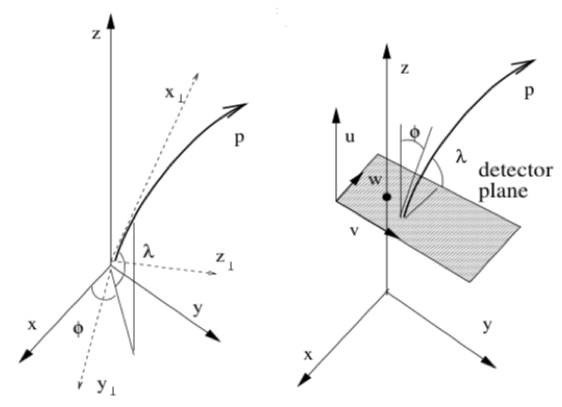
\includegraphics[width=0.5\textwidth]{FreeSurfaceSystems}
    \caption[Free and surface tracking coordinate systems]{Free (left) and surface (right) tracking coordinate systems.}
    \label{fig:FreeSurfaceSystems}
\end{figure}

\begin{figure}[]
  \centering
  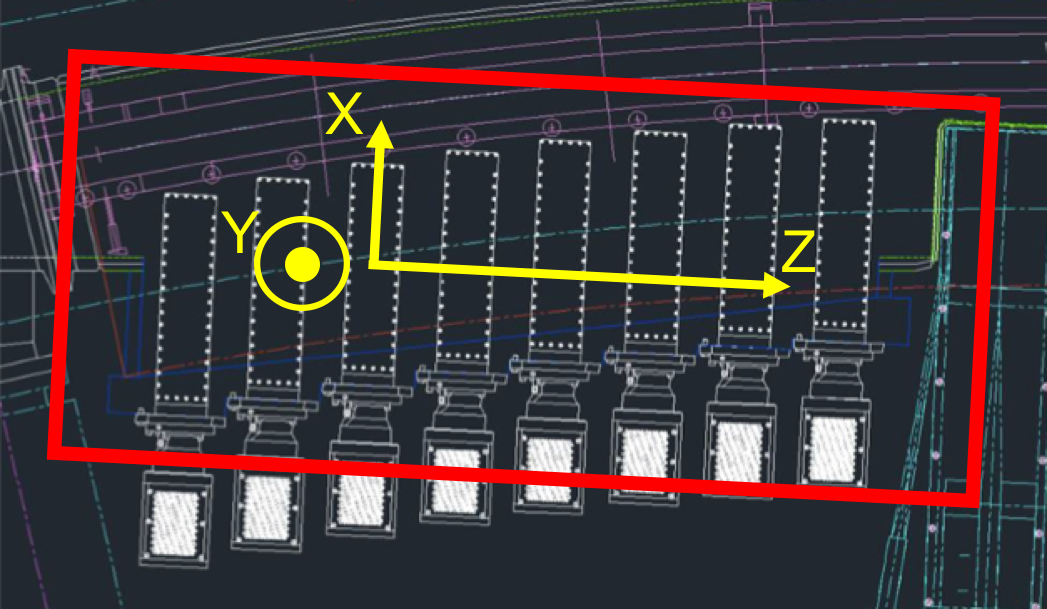
\includegraphics[width=0.7\textwidth]{trackerReferenceFrame}
    \caption[Tracker reference frame]{Shown is a model view of a tracker station in relation to the magnetic ring. Tracker modules are shown in white. Around the tracker measurement area is defined a coordinate system called the tracker reference frame. In that frame, the X coordinate is directed outward along the straws nearly radially, the Y coordinate is directed vertically up, and the Z coordinate is directed along the direction that the tracker modules are staggered.}
    \label{fig:trackerReferenceFrame}
\end{figure}


The $5 \times 5$ error matrix on a plane calculated in Geane describing the expected distribution in true parameters about the average ones is defined as
    \begin{align} \label{eq:errormatrix}
        \sigma_{N}^{ij} = <p_{N}^{i}p_{N}^{j}> - <p_{N}^{i}> \cdot <p_{N}^{j}>,
    \end{align} 
where i and j are track parameter indices and $N$ is some plane number. This error matrix will include effects from multiple scattering, delta ray production, ionization, and bremsstrahlung \cite{geanemanual,Lavezzi,energyloss}. These matrices are transported from plane to plane by what are called transport matrices, where the $5 \times 5$ transport matrix elements between two planes are defined as 
    \begin{align} \label{eq:transportmatrix}
        T_{N,N-1}^{i,j} = \frac{\partial p^{i}_{N}}{\partial p^{j}_{N-1}}.
    \end{align}
The transport matrix $T$ is a Jacobian between planes which expresses the infinitesimal changes in parameters at some plane (or path length) with respect to the parameters at some previous plane (or previous path length):
    \begin{align} \label{eq:parametertransport}
        \delta p_{N} &= T_{N,N-1} \delta p_{N-1}
    \end{align}
Note that the transport matrix does not propagate the track parameters themselves as with an equation of motion. The error matrix is propagated forward from one plane to another by
    \begin{align} \label{eq:errortransport}
        \sigma_{N} &= T_{N,N-1} \sigma_{N-1} T_{N,N-1}^{T} + \sigma_{\text{material}},
    \end{align}
where $\sigma_{\text{material}}$ is the added error due to material effects between the planes. See \figref{fig:FittingMatricesDiagram}. The calculation of the transport matrices themselves is done within the Geane routines in the free system on a step by step basis, where the derivation of the transport matrix elements is given in \refref{jacob}. It should briefly be pointed out that the transport matrix between any two planes (or number of steps) is the multiple of all intermediate transport matrices,
    \begin{align}
        T_{N,N-2} = T_{N,N-1} T_{N-1,N-2},
    \end{align}
regardless of what reference system the matrices are defined in (as long as they are all consistent). Geane can convert the transport matrices between the free system and the surface system using further Jacobians, also derived in \refref{jacob}. When converting a transport matrix from one reference system to another,
    \begin{align} \label{eq:Ttransform}
        T_{N,N-1}^{s} = A_{N} T_{N,N-1}^{f} A_{N-1}^{-1},
    \end{align}
where the $s$ and $f$ superscripts stand for the surface and free reference systems respectively, and $A$ is the Jacobian between reference frames which is defined at a specific point or plane $(A_{N} \neq A_{N-1})$. The error matrices are converted between reference frames in the usual way, 
    \begin{align} \label{eq:Sigtransform}
        \sigma_{N}^{s} &= A_{N} \sigma_{N}^{f} A_{N}^{T}.
    \end{align}


\begin{figure}[]
  \centering
  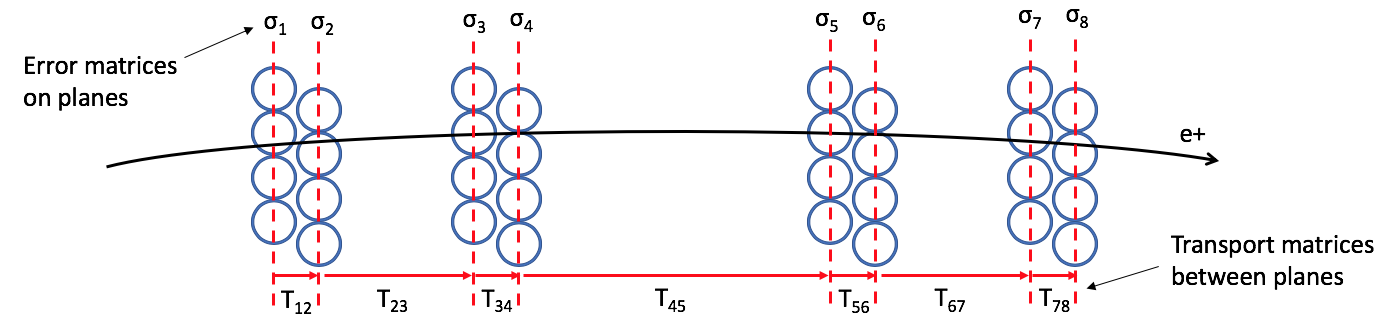
\includegraphics[width=\textwidth]{FittingMatricesDiagram}
    \caption[Transport and error matrices for straw tracker planes]{Transport matrices are defined between straw planes, and error matrices are defined on the planes.}
    \label{fig:FittingMatricesDiagram}
\end{figure}



Finally, while the tracker reference frame is nominally defined in the local XYZ coordinates as described previously, the straws themselves don't measure in that frame directly. As described in \secref{sec:StrawTrackers}, the straws measure drift circles in planes perpendicular to the straws themselves. The measurements from U and V straws therefore lie on the U and V measurement axes shown in \figref{fig:GeaneCoordSys}, where the measurement of the drift circle is instead taken as a U or V coordinate to the left or right of the straw wire. To first order the U or V coordinate is the DCA of the hit, which can be corrected with the angle of the track to get a better estimate, as shown in \appref{app:angularcorrection}. It's important to note that out of the five track parameters each straw only measures only a single U or V position. The new coordinate system is defined as
        \begin{align} \label{eq:trackermeasurementframe}
            \frac{1}{p}, \frac{p_{u}}{p_{z}}, \frac{p_{v}}{p_{z}}, u, v,
        \end{align}
where this $Z$ variable is the tracker reference frame $Z$, and the U and V coordinates here are non-orthogonal and are different to those in \equref{eq:UVW}. The transformation between the $XYZ$ and $UVZ$ systems is given by
    \begin{align}
        p^{UV} &= J_{5} p^{XY} \\
    \end{align}
where $J_{5}$ is a $5 \times 5$ matrix defined by
        \begin{align}
            J_{5} = 
            \begin{pmatrix}
                1 & 0 & 0 \\
                0 & J_{2} & 0 \\
                0 & 0 & J_{2}
            \end{pmatrix}
        \end{align}
and $J_{2}$ is a $2 \times 2$ matrix given by
        \begin{align}
            \begin{pmatrix}
                u \\
                v \\
            \end{pmatrix} =
            J_{2}
            \begin{pmatrix}
                x \\
                y \\
            \end{pmatrix} =
            \begin{pmatrix}
                \cos{\theta} & -\sin{\theta} \\
                \cos{\theta} & \sin{\theta} \\
            \end{pmatrix}
            \begin{pmatrix}
                x \\
                y \\
            \end{pmatrix}.
        \end{align}
$J_{2}$ is easily determined from \figref{fig:GeaneCoordSys}. In order to transform the transport or error matrices from the tracker reference frame to the tracker measurement frame, the same relations as in Equations~\ref{eq:Ttransform} and \ref{eq:Sigtransform} apply,
    \begin{align}
        T_{N,N-1}^{UV} &= J_{5} T_{N,N-1}^{XY} J_{5}^{-1} \\
        \sigma_{N}^{UV} &= J_{5} \sigma_{N}^{XY} J_{5}^{T}
    \end{align}
where the superscripts of $XY$ or $UV$ identify which coordinate system the objects belong to.

\begin{figure}[]
  \centering
  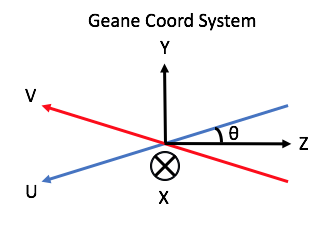
\includegraphics[width=0.5\textwidth]{GeaneCoordSys}
    \caption[Natural tracker measurement system]{The straw tracker measurement reference system. The XYZ system here is the straw tracker reference frame. $\theta$ is the same angle as the stereo angle of the straws, at 7.5\textdegree{}. U straws measure along the U axis and V straws measure along the V axis.}
    \label{fig:GeaneCoordSys}
\end{figure}




\subsection{\texorpdfstring{\chisq}{chisq} minimization}
\label{sec:TrackFittingAlgorithm}

% -cite james thing
% -it was found that doing the minimization in UV space removed correlations (cite James here) instead of XY, docdb 3813
% -performing the minimization in UV is most natural


The method for fitting and improving the track is a global \chisq minimization algorithm that uses the transport and error matrices as described previously \cite{geanemanual,trajfit}. This straightforward global fitting algorithm works because of the minimal amount of material contained within the tracker and the resulting small correlations between planes. For denser detectors with greater correlations, other fitting algorithms such as a Kalman filter should be used \cite{Lavezzi}. The following derivations and minimization assume measurements on planes in the tracker measurement frame described by \equref{eq:trackermeasurementframe}, but it should be noted that the results apply to any reference frame. A derivation for a \chisq including no material correlations is presented followed by one which includes said correlations.


The $\chi^{2}$ for a track is defined as the residuals between predicted and measured parameters on a measurement plane, divided by their errors, summed over all hit planes:
    \begin{align} \label{eq:chi2sum}
        \chi^2 = \sum_{i=1}^{N} [(p_{i}(p_{s})-x_{i})^{T} (\sigma_{i}^{-1}) (p_{i}(p_{s})-x_{i})]
    \end{align}
$x_{i}$ are vectors of the measured track parameters on plane $i$, $p_{i}$ are vectors of the average predicted track parameters which stem from some general starting parameters $p_{s}$, and $\sigma_{i}$ are the $5 \times 5$ error matrices on the plane\footnote{The vector $p_{s}$ has no numerical value at this time.}. To first order the error matrices consist only of the measurement errors on the U and V parameters and exclude the effects of random material processes. These errors are located in the U and V diagonal elements $(3,3)$ and $(4,4)$ respectively, with corresponding resolutions of \mum{150} as described in \secref{sec:StrawTrackers}. At second order the material error matrices as calculated by Geane are added to the measurement errors. Because the measured parameters consist of solely U or V measurements, the $x_{i}$ vectors are $5 \times 1$ objects where only the $(3)$ or $(4)$ elements have any meaning respectively\footnote{A straw tracker module as a whole can be approximated as measuring in 2D space, but this leads to correlations between measured parameters which must be taken into account, as compared to the natural tracker measurement frame in 1D space of U or V for which there are no measurement correlations \cite{UVcorrelations}. A fitting algorithm which fits the true measurement space of the drift circles themselves would be even better.}. The errors on the non-measured parameters in the diagonals of the error matrix are taken as infinite, such that when the error matrix is inverted all corresponding rows and columns of the final matrix on each plane reduce to zero and contribute nothing to the $\chi^{2}$.


By minimizing this \chisq with respect to the starting parameters $p_{s}$, and evaluating it at the target best starting guesses $p'_{0}$, which are the parameters of interest, the track can be fit:
    \begin{equation}
    \begin{aligned}
        \frac{\partial \chi^{2}}{\partial p_{s}}\Big|_{p_{s}=p'_{0}} = 0 
            &= \sum_{i=1}^{N}\Big[ \Big(\frac{\partial p_{i}(p_{s})}{\partial p_{s}}\Big|_{p_{s}=p'_{0}}\Big)^{T} (\sigma_{i}^{-1}) (p_{i}(p'_{0})-x_{i}) \\ 
            &+ (p_{i}(p'_{0})-x_{i})^{T} \Big(\frac{\partial(\sigma_{i}^{-1})}{\partial p_{s}}\Big|_{p=p'_{0}}\Big) (p_{i}(p'_{0})-x_{i}) \\ 
            &+  (p_{i}(p'_{0})-x_{i})^{T} (\sigma_{i}^{-1}) \Big(\frac{\partial p_{i}(p_{s})}{\partial p_{s}}\Big|_{p_{s}=p'_{0}}\Big)\Big]
    \label{eq:chi2summinimize}
    \end{aligned}
    \end{equation}
The middle term is small and can be neglected assuming that that the error matrix doesn't change much with respect to the choice of starting parameters. This is true as the error matrix is already small due to the low amount of material in the tracker. (In tandem the error matrix doesn't change much from one fitting iteration to the next as long as the path length through the material remains about the same.) The first and third terms are identical in value, and so must therefore both separately be equal to zero. \equref{eq:chi2summinimize} is therefore reduced to 
    \begin{align} \label{eq:chi2sumreduced}
        0 = \sum_{i=1}^{N} T^{T}_{i0} \sigma_{i}^{-1} (p_{i}(p'_{0})-x_{i}),
    \end{align}
where $T_{i0}$ is the transport matrix between the point at which the starting parameters are defined and plane $i$ given by \equref{eq:transportmatrix}:
    \begin{align} \label{eq:transportfrom0}
         T_{i0} = \frac{\partial p_{i}(p_{s})}{\partial p_{s}}\Big|_{p_{s}=p'_{0}}
    \end{align}
In minimizing the \chisq the desire is to update some original set of starting track parameters $p_{0}$ to the new best ones $p'_{0}$. This difference, $\Delta p_{0}$, can be determined by substituting the following equation into \equref{eq:chi2sumreduced},
    \begin{align} \label{eq:psub}
        p_{i}(p'_{0}) = p_{i}(p_{0}) + T_{i0} \Delta p_{0},
    \end{align}
which follows from \equref{eq:parametertransport}. After simplifying one arrives at 
    \begin{align} \label{eq:deltap}
        \Delta p_{0} = \sigma_{p_{0}} \sum_{i=1}^{N} T^{T}_{i0}(\sigma_{i}^{-1})(x_{i} - p_{i}(p_{0})),
    \end{align}
where
    \begin{align} \label{eq:cov}
        \sigma_{p_{0}} = [\sum_{i=1}^{N} T^{T}_{i0} (\sigma_{i}^{-1}) T_{i0} ]^{-1}.
    \end{align}
$\sigma_{p_{0}}$ is a $5 \times 5$ covariance matrix of the starting fit parameters, where the diagonals describe the fit errors in the 5 track parameters at that point. 
% \footnote{It should be noted that this minimization procedure does not supply the fit errors on each of the measurement planes, and only does so at the starting plane of the track.}

To summarize, an initial set of starting parameters $p_{0}$ are propagated forwards in Geane to produce predicted track parameters, transport matrices, and error matrices. These objects along with the measured parameters are plugged into the \chisq minimization algorithm detailed here to provide a \chisq describing the goodness of the fit corresponding to those original starting parameters, an improvement $\Delta p_{0}$ to those starting track parameters, and the errors $\sigma_{p_{0}}$ on those starting parameters. This consists of a single iteration of the track fitting. In order to determine the predicted parameters of the track corresponding to the improved starting parameters, the procedure needs to be repeated. The track fitting is iterated until the \chisq no longer improves, at which point the track fitting is said to have converged. Typically three or four iterations are enough to get a best fit track, as shown in \figref{iterationsfigure}. As a reminder the initial set of starting parameters is given by a circle fit to the hit straws as described at the end of \secref{sec:TrackFinding}. The starting parameters for a track are defined on a virtual $0$ plane parallel to the measurement planes, where the placement of the $0$ plane is defined based on a track by track basis and is placed at a point $\SI{1}{cm}$ in front of the first straw tracker module that was hit. Note that there is remarkable robustness with respect to the initial starting parameters in fitting the track. Of course if the initial starting parameters are too poor, then the fit will not converge. 







% could potentially show some results here


\subsection{Material correlations}


Random processes due to material contribute to the error matrix in \equref{eq:errormatrix} as described in \secref{sub:Geane}. The random scattering of a particle trajectory at one plane means that there is an extra error in all further planes. \equref{eq:chi2sum} does not take into account these material correlations between measurement planes when fitting the track. While this provides a decent approximation of the best fit track in the low material tracker, a better estimate of the track trajectory can be calculated. To do this a more general version of the \chisq equation can be used:
        \begin{align} \label{eq:chi2full}
            \chi^2 = (\vec{p}-\vec{x})^{T} (\sigma^{-1}) (\vec{p}-\vec{x}).
        \end{align}
Here $\vec{x}$ and $\vec{p}$ are a $5N \times 1$ vectors of the measured and predicted track parameters respectively, where $N$ is the number of planes hit, and these objects are the combined vectors of the corresponding objects in \equref{eq:chi2sum}. Similarly, $\sigma^{-1}$ is a $5N \times 5N$ matrix, where the $5 \times 5$ diagonal blocks are the individual plane error matrices described before, calculated between plane 0 and $N$. Solving for the \chisq is now recasted from a sum over measurement planes into a single large linear algebra equation. At this point both calculations of the \chisq's are equivalent.


The new format however allows for the material correlations between planes to be included, where these correlations are added as $5 \times 5$ matrices in the off-diagonal blocks of the new large error matrix. The upper diagonals are given by 
    \begin{align} \label{eq:corr}
        \sigma_{MN} = T_{MN} \sigma_{N}, 
    \end{align}
where $\sigma_{MN}$ is the material correlation matrix between plane $M$ and plane $N$, and $\sigma_{N}$ is still defined from \equref{eq:errortransport}, as calculated from the 0 starting plane. \textbf{Need to cite or prove this equation, should do the latter but I can't quite remember the derivation at the moment.} The lower diagonals are just the transpose of \equref{eq:corr}. The \chisq is minimized in the same way as was done in the previous section such that the improvement to the starting track parameters $\Delta p_{0}$ remains a $5 \times 1$ vector and is given by
    \begin{align} \label{eq:deltafull}
        \Delta p_{0} &= \sigma_{p_{0}} \tau^{T}\sigma^{-1}(\vec{x}-\vec{p}), \\
        \sigma_{p_{0}} &= [\tau^{T} \sigma^{-1} \tau ]^{-1},
    \end{align}
where $\tau$ is a $5N \times 5$ object of the individual transport matrices combined together.


In the inversion of the $5N \times 5N$ error matrix, the unmeasured parameter errors of infinity reduce all corresponding rows and columns to 0 in the same way as described before. Because these matrix objects are very large, where $N$ ranges from \SIrange{6}{32}{}, one can imagine that the inversion is a slow process. The tracking must have a certain amount of speed for the data to be efficiently processed and fit, which makes these inversions unfeasible. The solution used was to reduce the size of the $5N \times 5N$ matrix to an $N \times N$ one, simply by eliminating the rows and columns that would be sent to 0 anyways. The corresponding rows and columns of the unmeasured parameters in the combined transport matrix $\tau$ and $5N \times 1$ residual vector are also removed, resulting in an $N \times 5$ matrix for $\tau$ and an $N \times 1$ vector for the residuals. The covariance matrix $\sigma_{p_{0}}$ remains a $5 \times 5$ matrix as it should, and the final \chisq calculation is unaffected\footnote{Note that these element removals are done just before the final calculation of the \chisq and fit to the track and not at the beginning of the algebra, otherwise the plane material correlations are not properly included.}. Note that besides this $N \times N$ matrix inversion method, there is another way to do the inversion in a faster manner, which is described in \refref{trajfit}.



\clearpage % stopper for where I'm at 

    
% ($\sigma_{N}$ is the error matrix on plane N calculated from the starting plane.) This follows from equation \ref{eq:errormatrix} evaluated at plane M with respect to a path length from plane N, and not plane 0, which is equivalent to \ref{eq:corr}. 














\subsection{Truth/simulated fit results - fit to mc data}



\subsection{Left right ambiguity}
\label{sub:leftright}



\subsection{Plots and results and stuff}


% 3. Types of fitting used, various modes and options
%     1. Left-right ambiguity
% 4. Plots and images everywhere showing what all I've done


-go into all tests and pieces of the code
-vacuum fitting
-chi2 plot and overlayed red curve for x ndf
-checks on energy loss
-material correlation code
-fast fitting code
-different fitting modes
-mc / data comparisons
-don't forget about angular correction in appendix of fitting documentation - might want to put that in the appendix of my thesis
-red black point residual plots too maybe
-talk about the dummy stuff too perhaps
-ficticious starting plane


-should talk about geometry determination of hits in straws which I havent yet - in the fitting side of things though - see Joes docdb 6947 to start (maybe others too) - for LR determination after wire fit (but only in full sequence fit I believe...)



\subsection{In the code}

-should this be it's own section? should the picture be include at all? moved to the appendix?

Details of the track fitting code itself is described in \refref{trackfittingdoc}. 


\begin{figure}[]
  \centering
  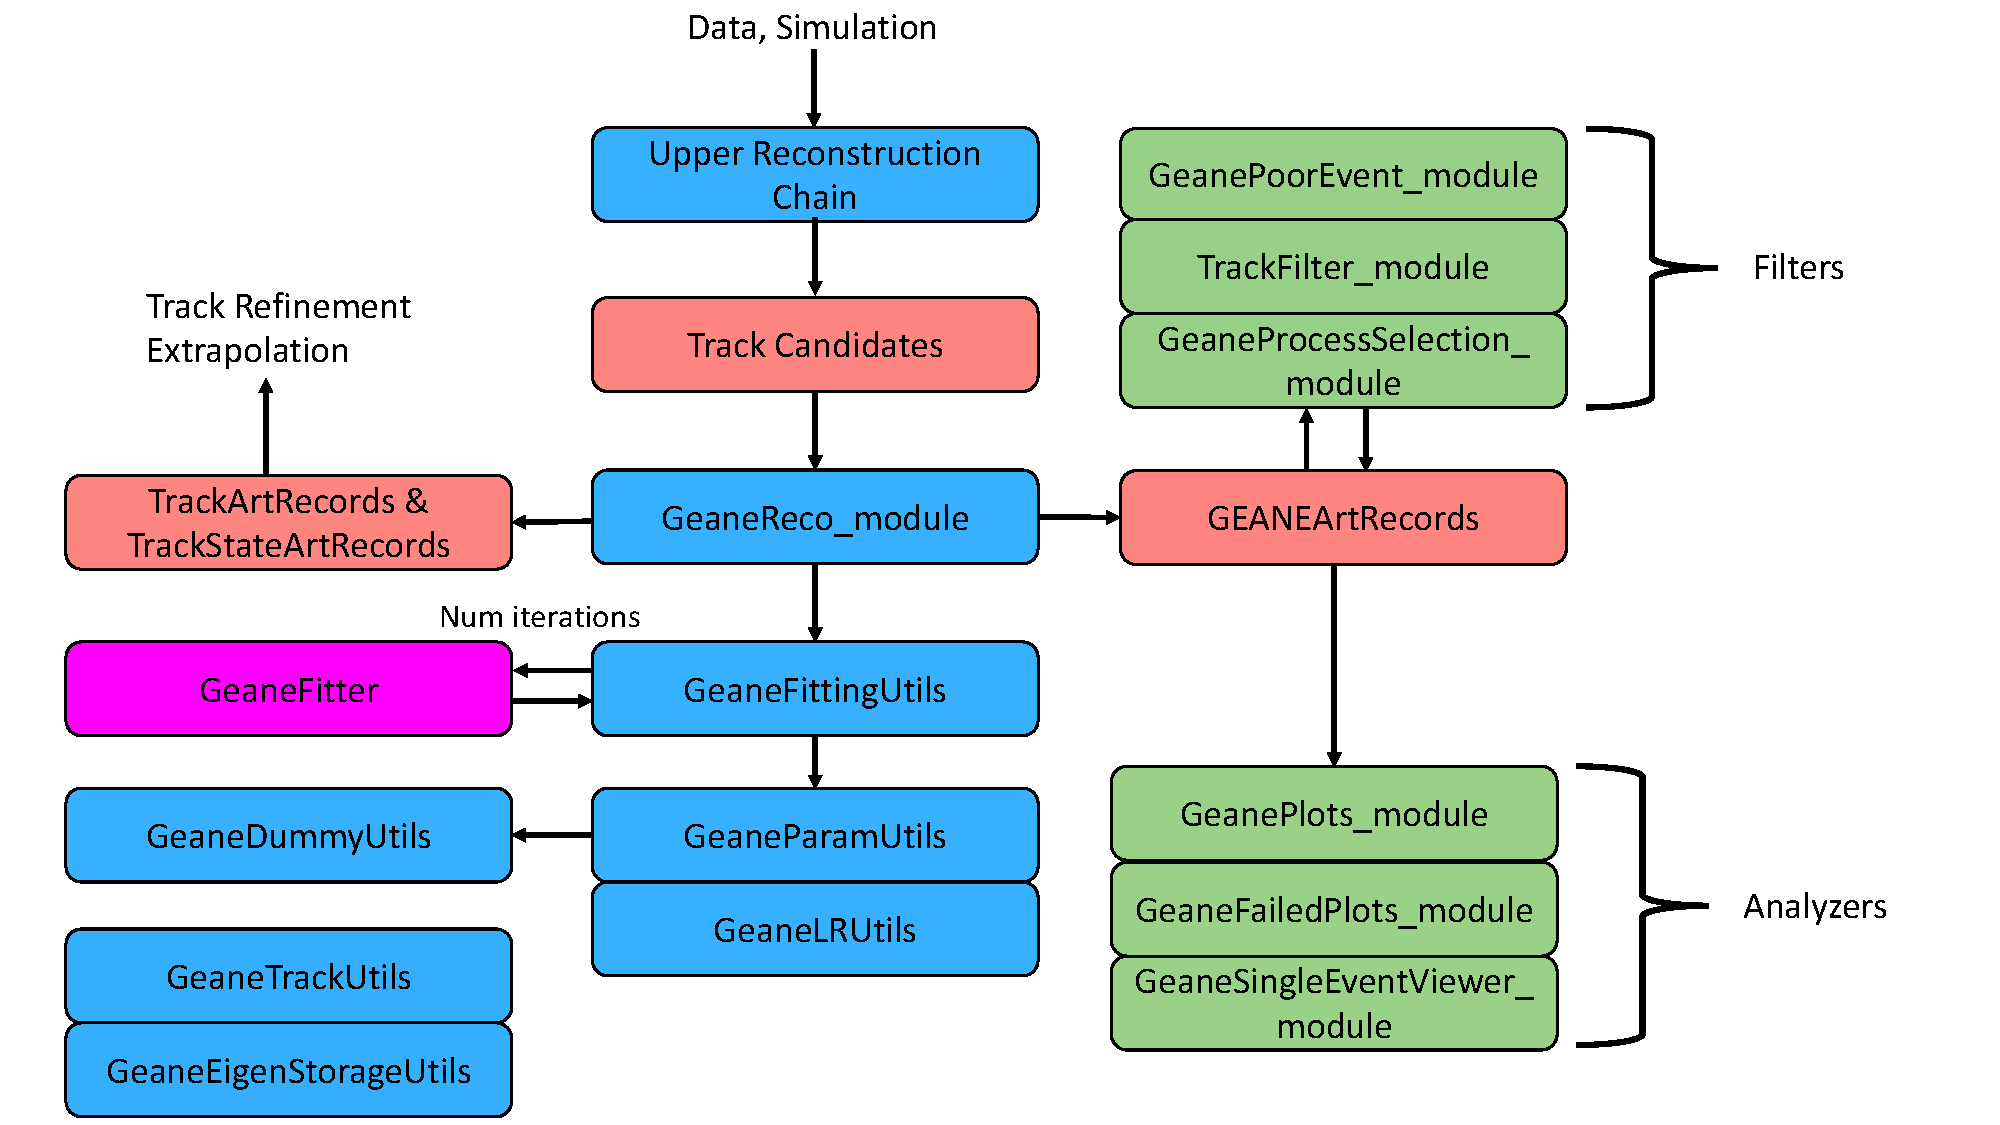
\includegraphics[width=\textwidth]{NewGeaneFlow}
    \caption[Geane code flow]{}
    \label{fig:NewGeaneFlow}
\end{figure}



\section{Track Extrapolation}
\label{sec:TrackExtrapolation}

The last stage of the track reconstruction is the track extrapolation. The extrapolation takes the fitted track results and either extrapolates them back to the storage region to the approximate position of the muon decay point, or forwards to the face of the calorimeter sitting right behind the tracker. The extrapolation stage utilizes a fourth order Runge-Kutta Nystr\"{o}m algorithm \cite{SCThesis} which discretely steps a trajectory through the magnetic field in the full \gmtwo Geant4 simulation, similar in some respects to the track fitting stage. At each step of the extrapolation, the updated track position and covariance matrix are compared to physical volumes in the simulation to flag tracks which have been reconstructed as likely originating from outside the storage region \cite{SCThesis,extrapolationerrors}. Because there is no fixed interaction point in the storage region, tracks are extrapolated backwards to the point of tangency where the radial momentum is equal to zero. Studies were done to verify that this approximation for the muon decay point was sufficient using truth Monte-Carlo, and it was found that a simple $\SI{1.1}{mm}$ correction to the radial decay position could be applied regardless of the momentum of the track \cite{SCThesis}. The vertical extrapolated distribution was found to have no biases. (What about the azimuthal point? Mentioned a little bit in DocDB 8564 but do I really want to go into it?) A birds eye view for extrapolation results is shown in \figref{fig:VertexPlanView}. A radial slice of the extrapolated beam distribution is shown in \figref{fig:BeamCrossSection}.


\begin{figure}[]
    \centering
    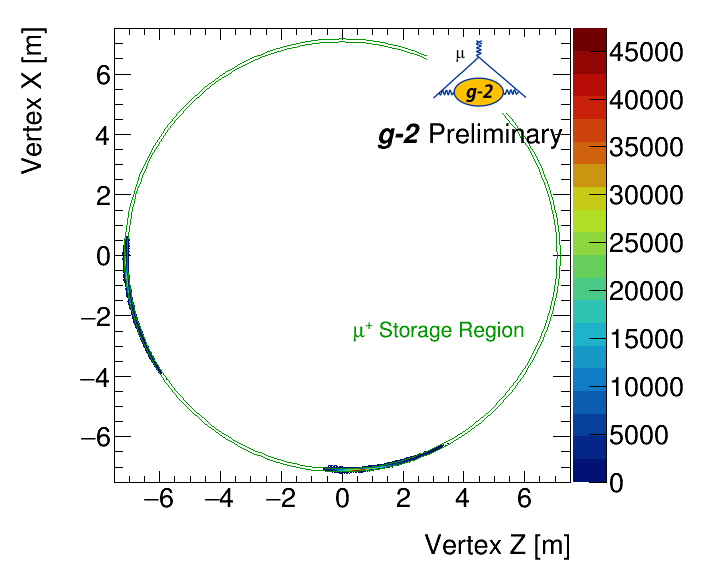
\includegraphics[width=\textwidth]{VertexPlanView}
    \caption[Birds eye view of extrapolation in ring]{A birds eye view of the extrapolation results in the storage ring. The two distributions of extrapolated tracks can be seen at the left and bottom of the figure, where the tracker sits at the heads of the distributions. It can be seen that some tracks are extrapolated multiple meters back through the storage region. (Mention anything about the cuts in this plot?)}    
    \label{fig:VertexPlanView}
\end{figure}

\begin{figure}[]
  \centering
  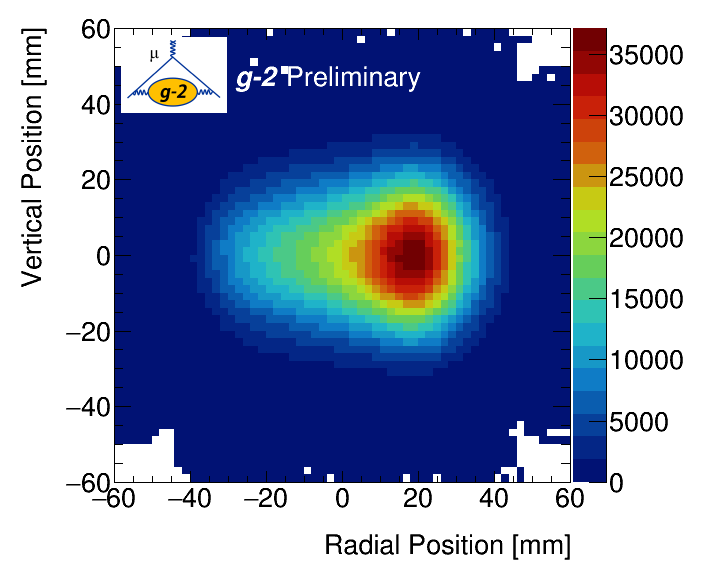
\includegraphics[width=0.7\textwidth]{BeamCrossSection}
    \caption[Extrapolated muon beam distribution cross-section]{Shown is a radial slice of the extrapolated muon distribution or beam spot. The beam is localized off center of the storage ring due to the kicker settings used, \secref{sub:kicker}. (Mention that last bit at all? Mention anything about the cuts in this plot?)}
    \label{fig:BeamCrossSection}
\end{figure}








\section{Muon Beam Measurements}
\label{sec:MuonBeamMeasurements}

-for showing plots include a bulleted list or table of the tracking cuts made

-emphasize measurements that are directly relevant to the calorimeter \wa analysis
-cbo frequency
-cbo amplitude
-have a CBO subsection alongside general results? 





\begin{figure}[]
    \centering
    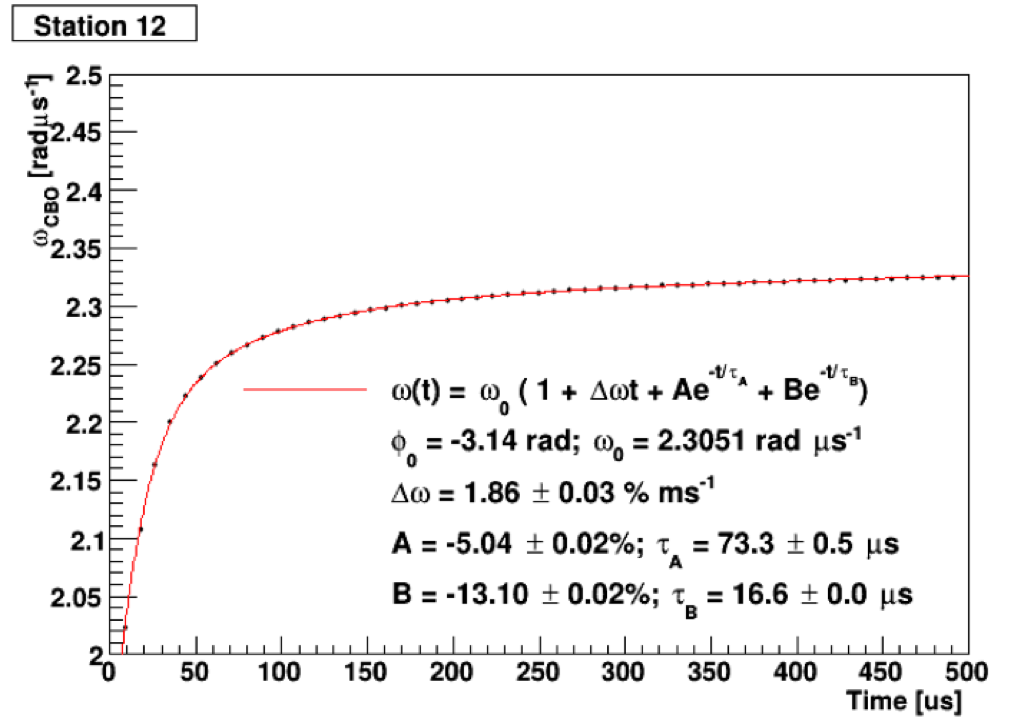
\includegraphics[width=0.9\textwidth]{CBOFrequency}
    \caption[CBO frequency]{}    
    \label{fig:CBOFrequency}
\end{figure}

\begin{figure}[]
    \centering
    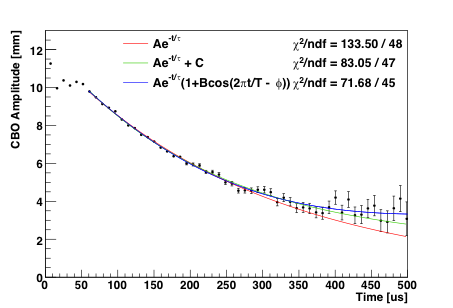
\includegraphics[width=0.9\textwidth]{CBOAmplitude}
    \caption[CBO amplitude]{}    
    \label{fig:CBOAmplitude}
\end{figure}



\clearpage


-in all pictures of this chapter (and others too), make sure to to go back through figures and check that I've given credit properly



